\chapter{Hardware design}

\section{Encoder}

\section{Højpasfilter}

\begin{figure}[htbp]
	\centering
	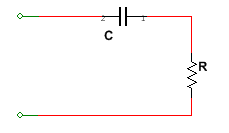
\includegraphics[width=0.50\textwidth]{billeder/HWdesign/HP_UV.png}
	\caption{Højpasfilter uden værdier.}
	\label{fig:HP_UV}
\end{figure}


\begin{align}
\label{eq: HP_networkfunction}T(s) = \frac{R}{R+\frac{1}{C \cdot s}} = \frac{\frac{1}{R \cdot C}}{\frac{1}{R \cdot C}+S} \cdot \frac{s}{\frac{1}{R \cdot C}} = \frac{\alpha}{s + \alpha} \cdot \frac{s}{K}         , K= \alpha
\end{align}

\begin{align}
	\omega_c = knækfrekvens \Rightarrow \omega_c = 120000 \cdot 2 \pi = 240000\pi 
\end{align} 

	Kondensatoren C vælges til 0,1$\mu$F  = 0,1 $\cdot$  $10^-6$ F

\begin{align}
	\frac{1}{R \cdot C} < 240000\pi \Rightarrow R > \frac{1}{240000\pi \cdot 0,1 \cdot 10^-6}
	\Rightarrow R > 13,62 \Omega
\end{align}
	R vælges til 14 $\Omega$

\begin{align}
	f_c (R=14\Omega) = \frac{\frac{1}{14 \cdot 0,1 \cdot 10^-6}}{2 \cdot \pi} =112,2kHz
\end{align}

\begin{figure}[htbp]
	\centering
	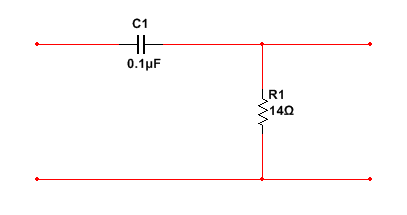
\includegraphics[width=0.50\textwidth]{billeder/HWdesign/HP_MV.png}
	\caption{Højpasfilter med værdier.}
	\label{fig:HP_MV}
\end{figure}

\newpage

\section{Zero Crossing Detector}

\newpage

\section{Båndpasfilter}

\subsection{Lavpasfilter}

\begin{figure}[htbp]
	\centering
	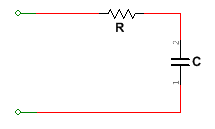
\includegraphics[width=0.50\textwidth]{billeder/HWdesign/LP_UV.png}
	\caption{Lavpasfilter uden værdier.}
	\label{fig:LP_UV}
\end{figure}


\begin{align}
\label{eq: LP_networkfunction}T(s) = \frac{\frac{1}{C \cdot s}}{\frac{1}{C \cdot s} + R} = \frac{\frac{1}{R \cdot C}}{\frac{1}{R \cdot C}+S}  = \frac{\alpha}{s + \alpha} , K= \alpha
\end{align}

\begin{align}
	\omega_c = knækfrekvens \Rightarrow \omega_c = 120000 \cdot 2 \pi = 240000\pi 
\end{align} 

Kondensatoren C vælges til 0,1$\mu$F  = 0,1 $\cdot$  $10^-6$ F

\begin{align}
	\frac{1}{R \cdot C} > 240000\pi \Rightarrow R < \frac{1}{240000\pi \cdot 0,1 \cdot 10^-6}
	\Rightarrow R < 13,62 \Omega
\end{align}
	R vælges til 13 $\Omega$
	
\begin{align}
	f_c (R=13\Omega) = \frac{\frac{1}{13 \cdot 0,1 \cdot 10^-6}}{2 \cdot \pi} =120,8kHz
\end{align}	
	
	
\begin{figure}[htbp]
	\centering
	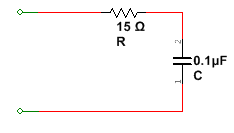
\includegraphics[width=0.50\textwidth]{billeder/HWdesign/LP_MV.png}
	\caption{Lavpasfilter med værdier.}
	\label{fig:LP_MV}
\end{figure}

\section{Buffer}

\section{Envelope Detector}
